\documentclass[tikz,10pt]{beamer}
\usepackage[utf8]{inputenc}
\usepackage[T1]{fontenc}
\usetheme{default}
\usepackage{lipsum}
\usepackage{listings}

% ----------------------------
% fabio - headers
% ----------------------------

\usepackage{tikz}
\usetikzlibrary{matrix,arrows.meta}

\setbeamertemplate{footline}[frame number]

\begin{document}
\author{Bruno Canale \\ Bruno Giordano \\ Fábio Sancinetti \\
  Wanderson Ferreira}
	\title{Estudos sobre Redes Neurais Convolucionais}
	\subtitle{Disciplina PSI5886 \\ Prof. Emilio Del
          Moral Hernandez}
	%\logo{}
	%\institute{}
	\date{\today}
	%\subject{}
	%\setbeamercovered{transparent}
	%\setbeamertemplate{navigation symbols}{}
        \maketitle
    \begin{frame}
	\frametitle{Objetivos do Trabalho}
	
	Os objetivos principais do trabalho foram:
	
	\begin{itemize}
	    \item Entender como as \textbf{MLPs} clássicas evoluíram para o que hoje é conhecido como Deep Learning
		\item Estudar a estrutura e o funcionamento de Redes Neurais
		Convolucionais 2D
		\item Entender como a informação é transformada dentro da
		rede neural ao avançar nas camadas mais profundas
		\item Extrapolar esse conhecimento para redes mais
		clássicas como a \textbf{MLP} estudada durante a
		disciplina.
	\end{itemize}
	\end{frame}

\begin{frame}
	\frametitle{Introdução e Motivação}
	\begin{itemize}
	\item Cybenko prova que uma rede neural MLP com uma camada escondida e com número arbitrário de neurônios consegue aproximar qualquer função
	
	\item Considerando tal resultado, por que tentar fazer redes neurais profundas?
	
	\item Delalleau e Bengio fizeram um estudo teórico \footnote{O. Delalleau, Y. Bengio - \emph{Shallow vs Deep Sum-Product Networks},
	\hskip 1em plus
	0.5em minus 0.4em\relax Neural Information Processing Systems} com neurônios simples (chamados de sum-product units) comparando a quantidade de neurônios necessária para uma aproximação com redes "superficiais" e "profundas"
	    
	\end{itemize}
	
\end{frame}

\begin{frame}
	\frametitle{Introdução e Motivação}
	\begin{itemize}
	\item De maneira simplificada, o trabalho \footnote{O. Delalleau, Y. Bengio - \emph{Shallow vs Deep Sum-Product Networks},
	\hskip 1em plus
	0.5em minus 0.4em\relax Neural Information Processing Systems} conclui que, para uma classe de funções:
	
	\textbf{It shows that some deep sumproduct network with n inputs and depth $O(\log{n})$ can represent with $O(n)$ units what would require $O(2^{\sqrt{n}})$ units for a depth-2 network.}
	\item Em outras palavras, conclui-se que para alguns tipos de funções a utilização de redes neurais como postuladas por Cybenko requer um número de neurônios consideravelmente maior à uma rede neural com mais camadas escondidas
	\item Tarefas clássicas de inteligência artificial (como reconhecimento de imagens) se encaixam em algumas dessas premissas, justificando a utilização de arquiteturas profundas nesses problemas
	 
	\item O que acontece se aumentarmos arbritariamente o número de camadas escondidas em uma MLP clássica como visto em aula?

	\end{itemize}
	
\end{frame}


\begin{frame}
    \frametitle{Análise preliminar da MLP clássica vista em sala}
 
     Para entender os problemas no aprendizado de redes com grande número de camadas escondidas em uma MLP clássica, vamos relembrar alguns conceitos de rede neurais com a arquitetura profunda mais simples possível \footnote{Michael A. Nielsen. - \emph{Neural Networks and Deep Learning},
	\hskip 1em plus
	0.5em minus 0.4em\relax Determination Press, 2015} :
    
    
    \begin{figure}
	\centering
	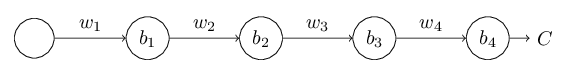
\includegraphics[scale=0.5]{nnetsimples.png}
	\end{figure}
	Seja $a_i$ o output do i-\'esimo neur\^onio do modelo. Ou seja:

$$a = \begin{cases}
a_1 = \sigma\big( w_1 x + b_1\big) = \sigma( z_1 ) \\
a_i = \sigma\big( w_i a_{i-1} + b_i\big) = \sigma( z_i ) \enspace \enspace i>1
\end{cases}$$

Onde $\sigma(.)$ \'e a fun\c{c}\~ao de ativa\c{c}\~ao do i-\'esimo neur\^onio.
	A derivada parcial de $C$ em relação à $w_1$ pode ser calculada como:
	
	$$ \frac{\partial C}{\partial w_1} = x \cdot \sigma^{'}(z_1) \cdot w_2 \cdot \sigma^{'}(z_2) \cdot w_3 \cdot \sigma^{'}(z_3) \cdot w_4 \cdot  \sigma^{'}(z_4)\cdot\frac{\partial C}{\partial a_4}$$
    
\end{frame}

\begin{frame}
	\frametitle{Análise preliminar da MLP clássica vista em sala}
	Há dois problemas cruciais consequentes da expressão da derivada parcial de $C$ em relação à $w_1$.
	
	\begin{itemize}
	    \item Função de perda $C$:
	    
	    $C = \frac{(y - a_4)^2}{2}$ como erro quadrático médio não é muito adequado para problemas de classificação:
	    $$ \frac{ \partial C } {\partial w_4 } = a_3(a_4 - y_{ref})\sigma^{'}(z_4)$$
	    
	    Para $a_4 \rightarrow \{1,0\}$, $\sigma^{'}(z_4) \rightarrow 0$. Assim, se $a_4 \rightarrow \{1,0\}$, $ \frac{ \partial C } {\partial w_4 } \rightarrow 0$. Se $a_4 \rightarrow y_{ref}$, é interessante que os pesos se modifiquem menos pois $a_4$ já está correto. Entretanto, se $a_4$ estiver próximo do valor binário contrário à $y_{ref}$, $\sigma^{'}(z_4)$ impede uma correção grande nos pesos para corrigir $a_4$.
	    
	    Alternativa: Cross-Entropy Loss
	   
	\end{itemize}
\end{frame}

\begin{frame}
	\frametitle{Análise preliminar da MLP clássica vista em sala}
    	
    	Cross-entropy loss:
    	
    	$C = - \bigg(y_{ref} \ln{a_4} + (1-y_{ref}) \ln{(1 - a_4)} \bigg)$
    	
    	Como $y_{ref} = \{1,0\}$, podemos perceber que $C \rightarrow 0$ se $a_4 = y_{ref}$ e $C \rightarrow \infty$ se $a_4$ se aproxima do valor binário contrário de $y_{ref}$. A propriedade mais interessante dessa função de perda está em sua derivada parcial:
    	
    	$$\frac{ \partial C } {\partial w_4 } = a_3(a_4 - y_{ref})$$
    	
    	Como podemos ver, a derivada independe de $\sigma^{'}(z_4)$. Assim, não há mais o problema mencionado anteriormente. Nas implementações práticas percebe-se que tal função de perda resulta em um treinamento consideravelmente mais rápido para problemas de classificação. Note que esse problema não é especificamente relacionado à redes profundas já que só se manifesta na última camada. Experimentalmente, verificou-se que para arquiteturas profundas diferentes camadas aprendiam em taxas diferentes de acordo com sua profundidade. Vamos voltar a analisar $\frac{\partial C}{\partial w_1}$:
    	

\end{frame}

\begin{frame}
	\frametitle{Análise preliminar da MLP clássica vista em sala}
	 Considere $\frac{\partial C}{\partial w_1}$:
	 
	$$ \frac{\partial C}{\partial w_1} = x \cdot \sigma^{'}(z_1) \cdot w_2 \cdot \sigma^{'}(z_2) \cdot w_3 \cdot \sigma^{'}(z_3) \cdot w_4 \cdot  \sigma^{'}(z_4)\cdot\frac{\partial C}{\partial a_4} \rightarrow $$
	$$ \frac{\partial C}{\partial w_1} = x \bigg(w_2 w_3 w_4 \bigg) \cdot \bigg(\sigma^{'}(z_1) \cdot \sigma^{'}(z_2)\cdot \sigma^{'}(z_3) \cdot \sigma^{'}(z_4) \bigg) \frac{\partial C}{\partial a_4} $$
	
	Sabemos que para $\sigma(z) = \frac{1}{1 + e^z}$, $\sigma^{'}(z) \leq 0.25$ e que $\sigma^{'}(z) \rightarrow 0$ para certos valores de $z$. Assim, a multiplicação de vários $\sigma^{'}(z)$ resulta em valores cada vez menores. Quanto maior a "distância" entre a camada e a função de perda $C$, menor a velocidade de aprendizado. Em particular, se inicializarmos todos os pesos com a mesma distribuição aleatória sem considerar a profundidade da camada em que se encontram, teremos uma inicialização com $\frac{\partial C}{\partial w_1} < \frac{\partial C}{\partial w_2} < \frac{\partial C}{\partial w_3} < ... $ . Tal problema é uma das principais causas da convergência para mínimos locais em redes profundas, comumente chamado na literatura de \it{Vanishing Gradient Problem}.
	
\end{frame}

\begin{frame}
	\frametitle{Deep Learning}
	Durante um bom tempo tal problema impossibilitava a utilização de arquiteturas profundas para machine learning. Em 2006 \footnote{Hinton et al. - \emph{A fast learning algorithm for deep belief nets},
	\hskip 1em plus
	0.5em minus 0.4em\relax Neural Computation, 2006} e 2007 \footnote{
	Bengio et al. - \emph{Greedy Layer-Wise Training of Deep Networks},
	\hskip 1em plus
	0.5em minus 0.4em\relax Neural Information Processing Systems, 2007} surgiram os primeiros algoritmos bem sucedidos para lidar com esse problema objetivando melhorar a inicialização da rede.
	
	Ambos algoritmos exploravam a ideia da utilização de técnicas de aprendizado não supervisionado para a inicialização dos pesos da rede seguidas de técnicas de aprendizado supervisionado. Tal estratégia talvez não seja mais tão utilizada atualmente em classificadores estado-da-arte, mas certamente foi extremamente importante na época pois estimulou a comunidade científica na pesquisa de novos métodos para treinamento de redes profundas.
	
	Surge, assim, o Deep Learning como conjunto de técnicas para melhorar o treinamento de redes profundas. Indicaremos a seguir algumas técnicas já consolidadas:
	
\end{frame}


\begin{frame}
	\frametitle{Regularização}
	Como vimos, o problema de aprendizado lento ocorre quando $\frac{\partial C}{\partial w_i}$ é pequeno. Considerando $\sigma(z)$ e $\sigma^`(z)$, sabemos que isso ocorre criticamente quando o módulo de $z$ é grande. Já que $z = \vec{w}^T \vec{a} + b$ (onde $\vec{a}$ são as ativações da camadas anterior e portanto são menores ou iguais a 1), o módulo de $z$ é grande quando o módulo de $\vec{w}$ é grande.
	
	Assim, para evitar que a rede "caminhe" durante o treinamento para regiões de baixo aprendizado, introduzimos um termo na função de custo C que penaliza pesos grandes. Por exemplo, a regularização L2 utiliza a norma L2 dos pesos $\vec{w}$ como penalidade:
	
	$$C_{reg} = C_{orig} + \lambda \vec{w}^T \vec{w}$$
	
	Onde o parâmetro $\lambda$ é utilizado como hyper-parâmetro para ponderar a importância desse termo na função de perda. Quanto maior o parâmetro $\lambda$, menores serão os pesos encontrados durante o treinamento.
	
\end{frame}


\begin{frame}
	\frametitle{Dropout}
    Introduzido por Hinton et al. \footnote{
	Hinton et al. - \emph{Improving neural networks by preventing
co-adaptation of feature detectors},
	\hskip 1em plus
	0.5em minus 0.4em\relax 2012}, pode ser interpretado simplificadamente como uma técnica para evitar o problema de overfitting. Em cada iteração de treino, há uma probabilidade $p$ para cada neurônio estar ativo (pesos $w$ mantidos) e (1-p) de estar inativo (pesos $w$ zerados). 
	
	 \begin{figure}
	\centering
	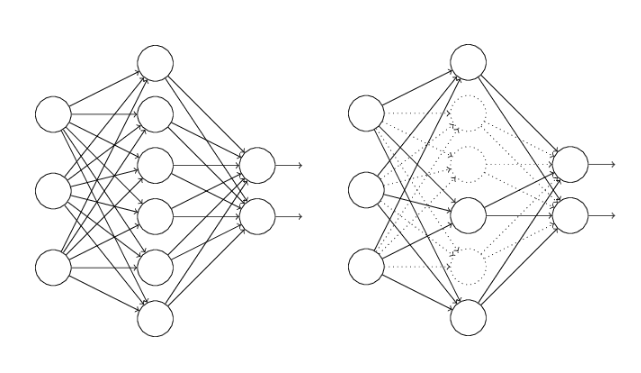
\includegraphics[scale=0.3]{dropout.png}
	\end{figure}
	
	Foi popularizada após a utilização de Krizhevsky et al. \footnote{
	Krizhevsky et al. - \emph{ImageNet Classification with Deep Convolutional Neural Networks}
	\hskip 1em plus
	0.5em minus 0.4em\relax 2012} em sua solução campeã da competição ImageNet de 2012. 
	\tiny{\it{"This technique reduces complex co-adaptations of neurons, since a neuron cannot rely on the presence of particular other neurons. It is, therefore, forced to learn more robust features that are useful in conjunction with many different random subsets of the other neurons."}}
	
\end{frame}


\begin{frame}
	\frametitle{Generalização de arquiteturas de ativação: building blocks}
	
Com o passar dos anos, a comunidade científica foi testando experimentalmente novas metodologias orientadas à     resultados sem tanto embasamento teórico como a MLP de Cybenko. Nesse contexto, novas funções de ativação e       novas arquiteturas de conexões entre neurônios foram surgindo na tentativa de inserir conhecimento específico     de domínio na generalidade das redes neurais. Introduz-se então o conceito de "building blocks", que são pequenos blocos neurais pré-definidos.

Alguns exemplos:

	 \begin{figure}
	\centering
	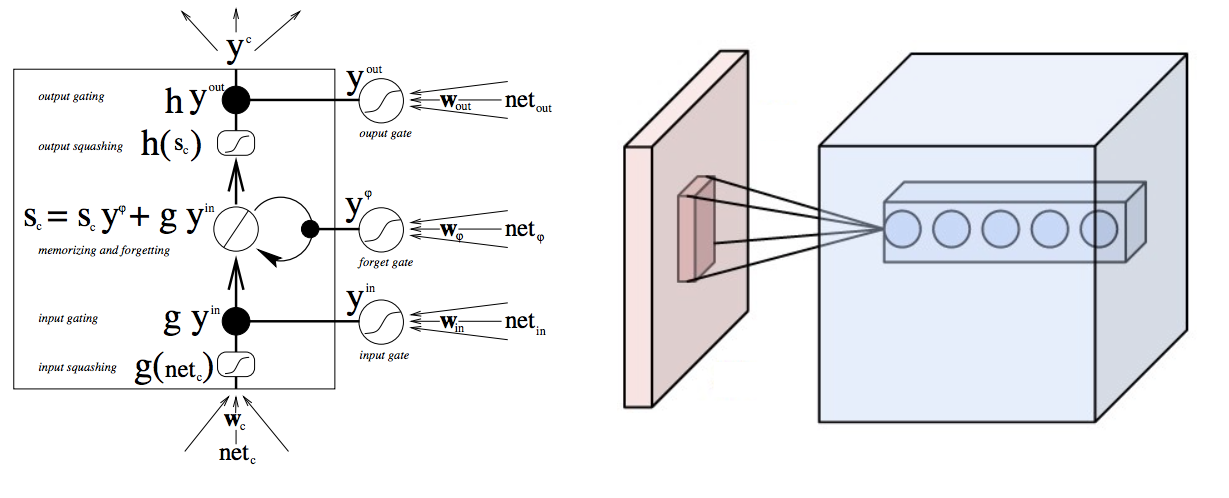
\includegraphics[scale=0.3]{blocks.png}
	\end{figure}
	
	
\end{frame}

\begin{frame}
	\frametitle{Apresentação do Bruno Canale}
\end{frame}


\begin{frame}
	\frametitle{Visualizando a Convolução}
	\centering
	\par \url{http://setosa.io/ev/image-kernels/}
	\par Explicação visual sobre Convoluções com demonstrações em Javascript
\end{frame}


\begin{frame}
	\frametitle{Python - Keras Framework para Machine Learning}
	
	* Python - Linguagem de programação gratuita \newline
	* Contém uma quantidade muito grande de Frameworks voltados para
	\textit{Machine Learning}
	
	
	\begin{figure}
		\centering
		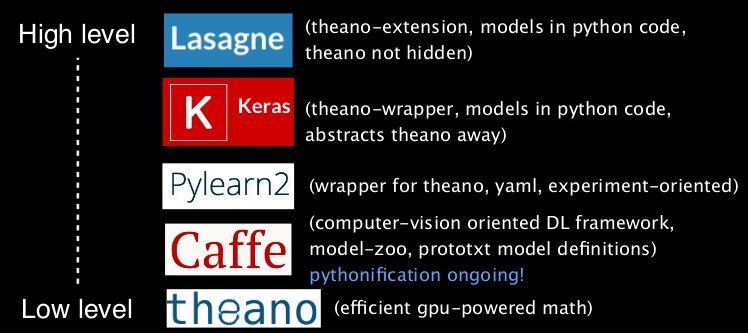
\includegraphics[scale=0.3]{road_map}
	\end{figure}
	
	Keras foi inicialmente desenvolvido como parte de um projeto de
	pesquisa chamado de ONEIROS (Open-ended Neuro-Electronic
	Intelligent Robot Operating System)
	
\end{frame}

\begin{frame}
	\frametitle{Keras - Exemplo de implementação MLP}
	
	
	modelo = Sequential() \\
	modelo.add(Dense(num-neuronios, init='uniform'))\\
	modelo.add(Activation('tanh')) \newline
	
	modelo.add(Dense(1, init='uniform')) \\
	modelo.add(Activation('linear')) \newline
	
	modelo.compile(learning-rate=0.1, optimizer='sgd]') \newline
	
	modelo.fit(features-treino, target-treino) \newline
	
	modelo.predict(features-teste)
	
\end{frame} 

\begin{frame}
	\frametitle{Base de dados utilizada - MNIST}
	
	\begin{columns}
		\begin{column}{0.48\textwidth}
			A base de dados MNIST é composta por 60.000 exemplos de
			imagens de digitos em letra cursivas. O dataset é ideal para
			testes de algoritmos em reconhecimentos de padrões por
			necessitar pouco pré-processamento.\\
			Mais informações no link: http://yann.lecun.com/exdb/mnist/
		\end{column}
		\begin{column}{0.48\textwidth}
			\begin{figure}
				\centering
				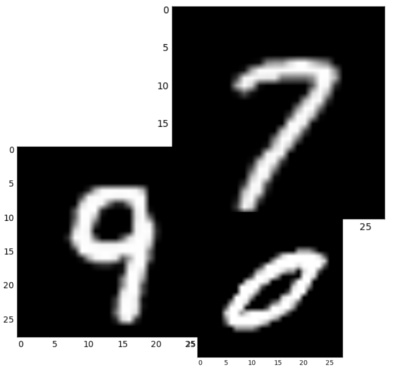
\includegraphics[scale=0.35]{minst}
			\end{figure}
		\end{column}
	\end{columns}
	
	\lstinputlisting[language=Python, firstline=0, lastline=10,
	basicstyle=\ttfamily\scriptsize]{base_import.py}
\end{frame}

\begin{frame}
	\frametitle{Processamento necessário no atributo target}
	
	Um processamento padrão é transformar o conjunto de
	\textbf{atributos targets} em um conjunto de variáveis
	categóricas. O que seriam variáveis categoricas?
	
	Exemplo: Se a lista de targets é composta por: [1.2, 2, 3, 4.2,
	4i] e as classes disponiveis são \textbf{real, inteiro,
		imaginario}, então uma matriz de transformação seria:
	
	\begin{table}[h]
		\caption{Conversão para variáveis categoricas}
		\begin{tabular}{l|c|c|c|}
			
			target & real & inteiro & imaginario \\
			1.2    & 1    & 0       & 0 \\
			2      & 0    & 1       & 0 \\
			3      & 0    & 1       & 0 \\
			4.2    & 1    & 0       & 0 \\
			4i     & 0    & 0       & 1
			
		\end{tabular}
	\end{table}
\end{frame}

\begin{frame}
	\frametitle{Implementação da Rede Convolucional 2D}
	\lstinputlisting[language=Python, firstline=0, lastline=25,
	basicstyle=\ttfamily\scriptsize]{cnn1.py}
\end{frame}

\begin{frame}
	\frametitle{Modelo do Experimento realizado para análise da
		Rede}
	\begin{itemize}
		\item Após implementação a arquitetura foi testada para
		verificar performance no conjunto de testes.
		\item Queriamos observar a transformação da imagem de Input
		após cada camada da ConvNet
		\item A fim de analisar com mais detalhes, foram adicionadas
		mais camadas convolucionais no modelo apresentado anteriormente.
	\end{itemize}
\end{frame}

% -------------------------------------------------
% \begin{fabio}
% -------------------------------------------------

\begin{frame}
	\frametitle{Redes e Resultados}

    \begin{figure}
	\centering
	\begin{minipage}{.33\textwidth}
		\centering
		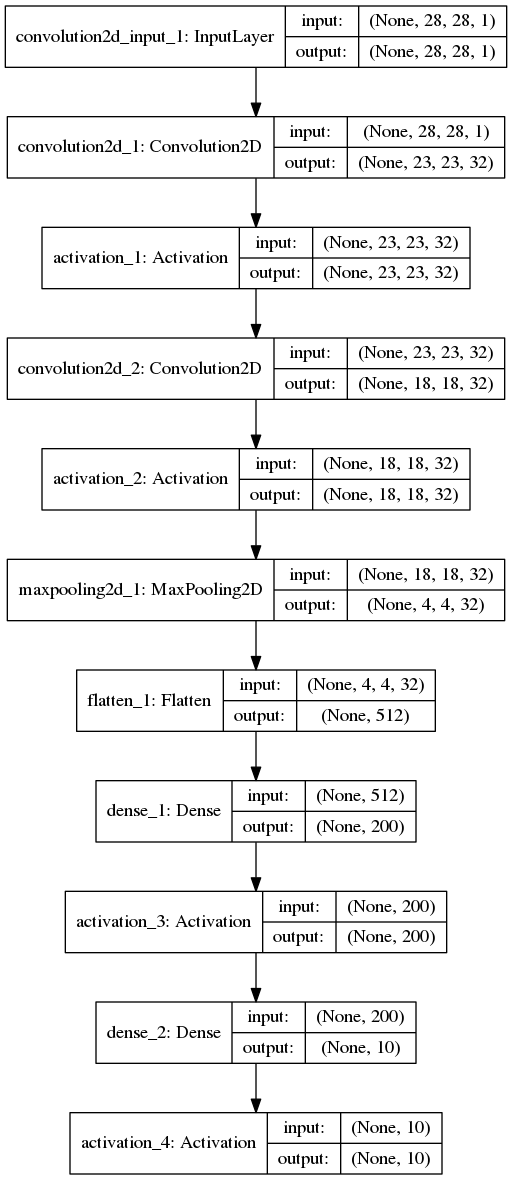
\includegraphics[width=.4\linewidth]{images/resultados/default/model}
	\end{minipage}%
	\begin{minipage}{.33\textwidth}
		\centering
		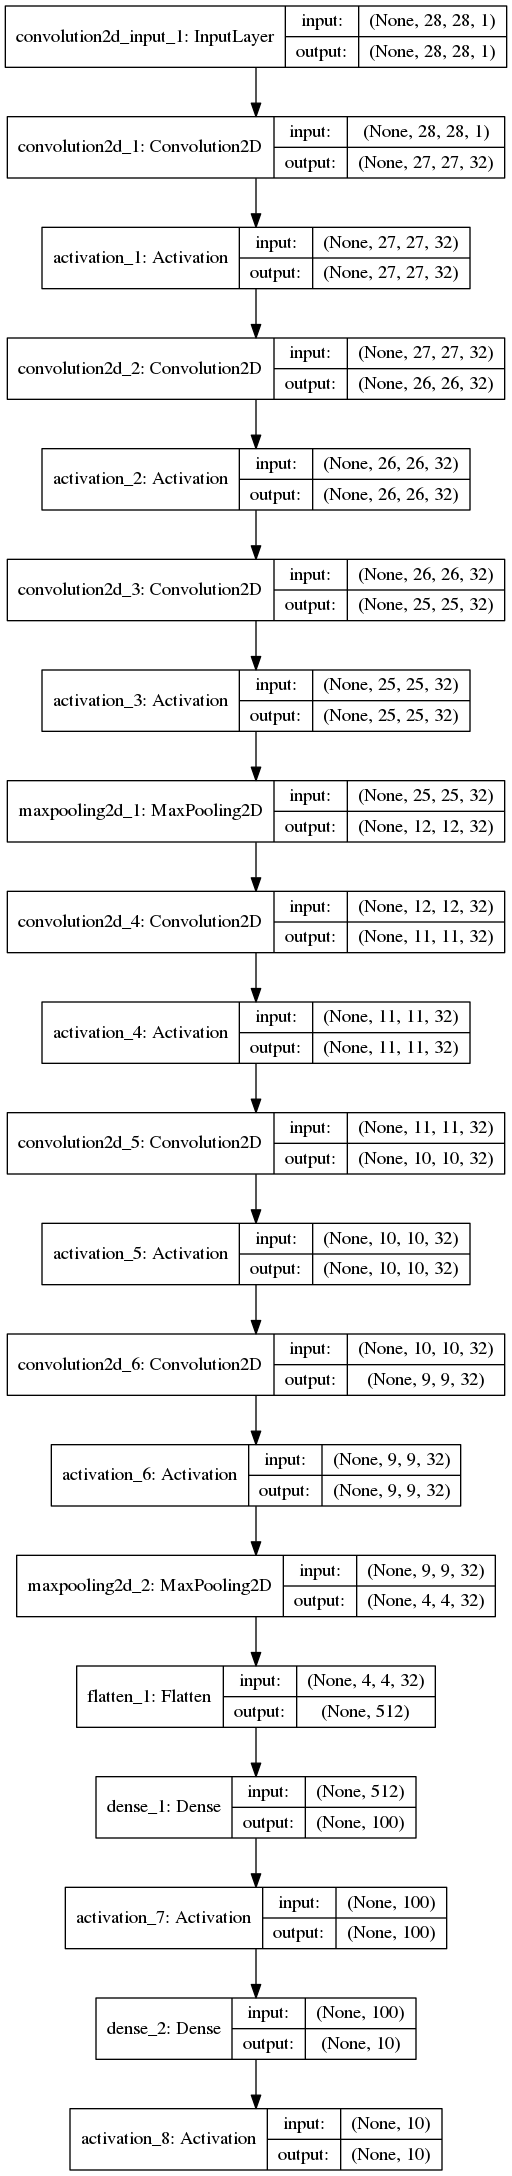
\includegraphics[width=.4\linewidth, height=.9\textheight]{images/resultados/network_1/model}
	\end{minipage}%
	\begin{minipage}{.34\textwidth}
	\centering
	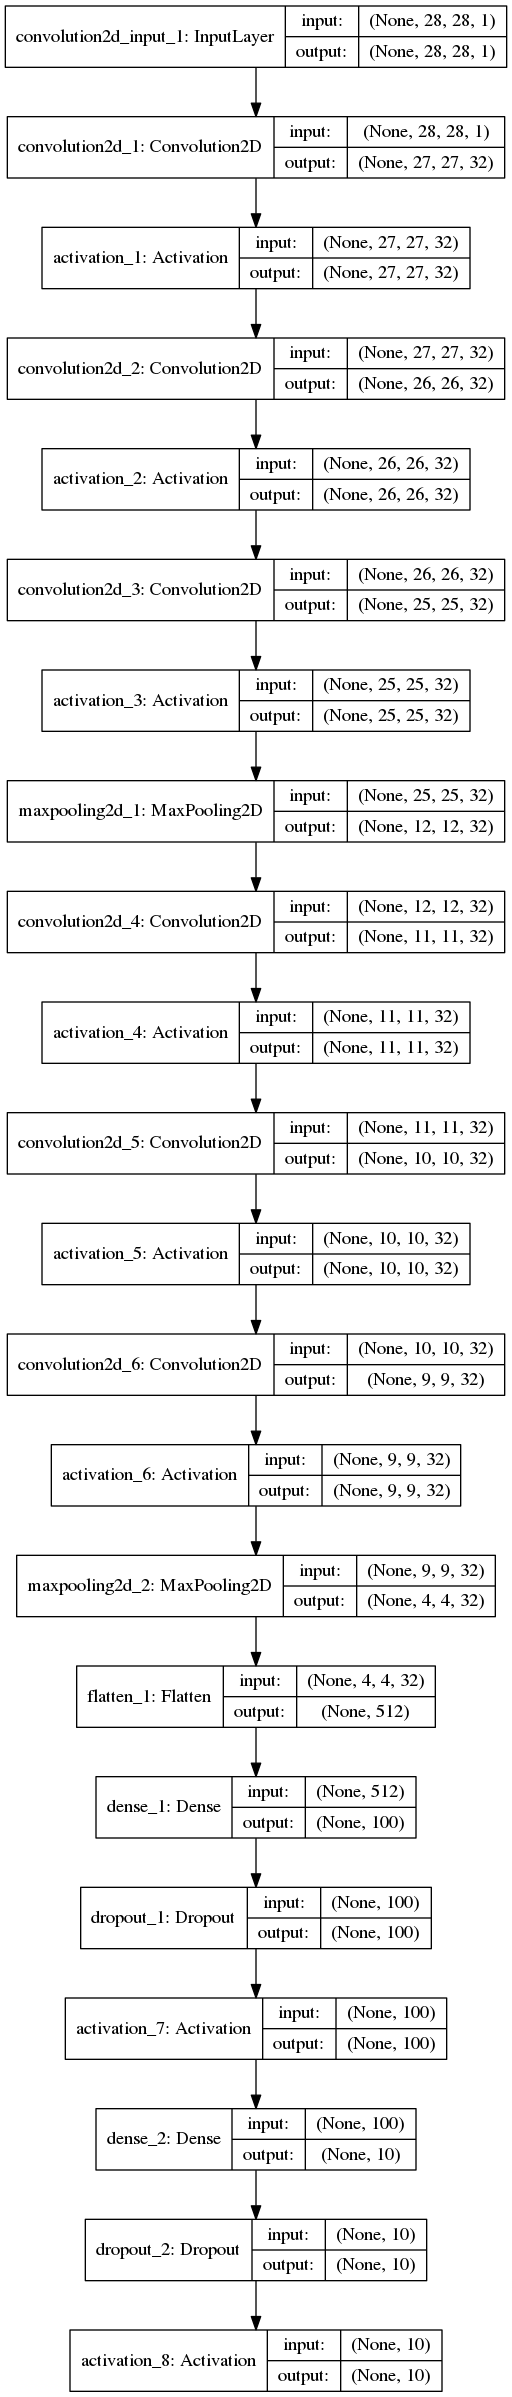
\includegraphics[width=.4\linewidth, height=.9\textheight]{images/resultados/network_2/model}
	\end{minipage}

\end{figure}

\end{frame}


\begin{frame}
	\frametitle{Camada de entrada}
	\centering
	MNIST DATASET
	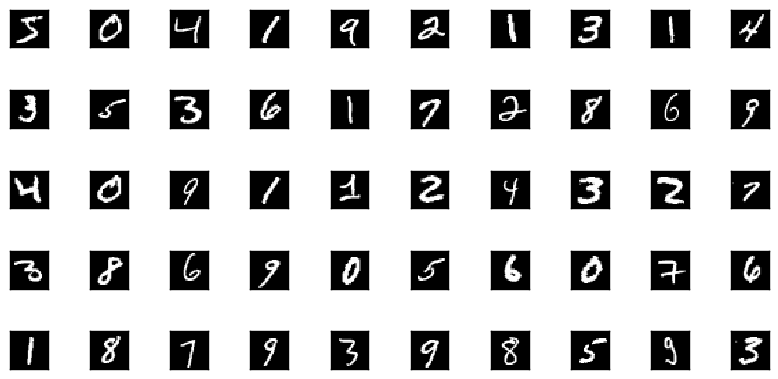
\includegraphics[width=.8\paperwidth]{images/fabio/inputs}
\end{frame}

\begin{frame}
	\frametitle{Aplicação da CNN}
	\centering
	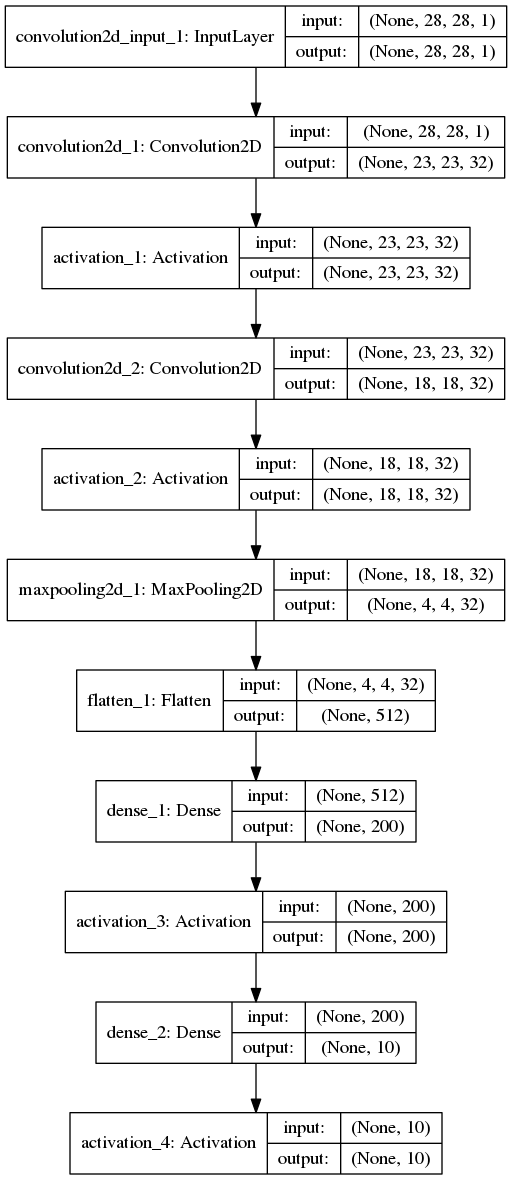
\includegraphics[height=.8\paperheight]{images/resultados/default/model}
\end{frame}

\begin{frame}
	\frametitle{Treinamento}
	\centering
%	\begin{minipage}{.5\textwidth}
		\centering
		\par Treinamento
		\begin{itemize}
			\item Épocas = 10
			\item Itens = 60000
			\item Tempo = 30 ~ 40 minutos
		\end{itemize}		
%	\end{minipage}%
%	\begin{minipage}{.5\textwidth}
	\centering
	\par Teste
	\begin{itemize}
		\item Itens = 10000
	\end{itemize}		
	\centering
	\par Resultado na base de teste
	\begin{itemize}
		\item 98.02\%
	\end{itemize}
%\end{minipage}%

\end{frame}

\begin{frame}
	\frametitle{Convolução - 1}
	\centering
	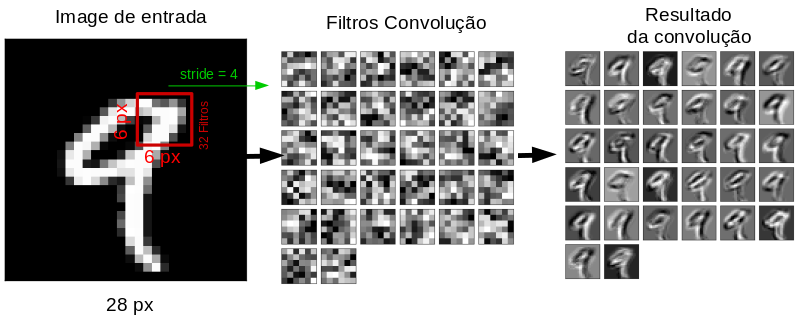
\includegraphics[width=.8\paperwidth]{images/fabio/conv_1}
\end{frame}

\begin{frame}
	\frametitle{Ativação - 1}
	\centering
	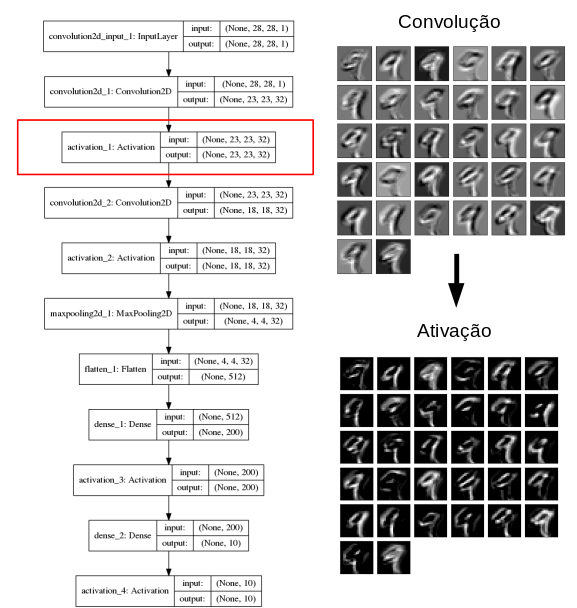
\includegraphics[height=.8\paperheight]{images/fabio/ativ_1}
\end{frame}

\begin{frame}
	\frametitle{Convolução - 2}
	\centering
	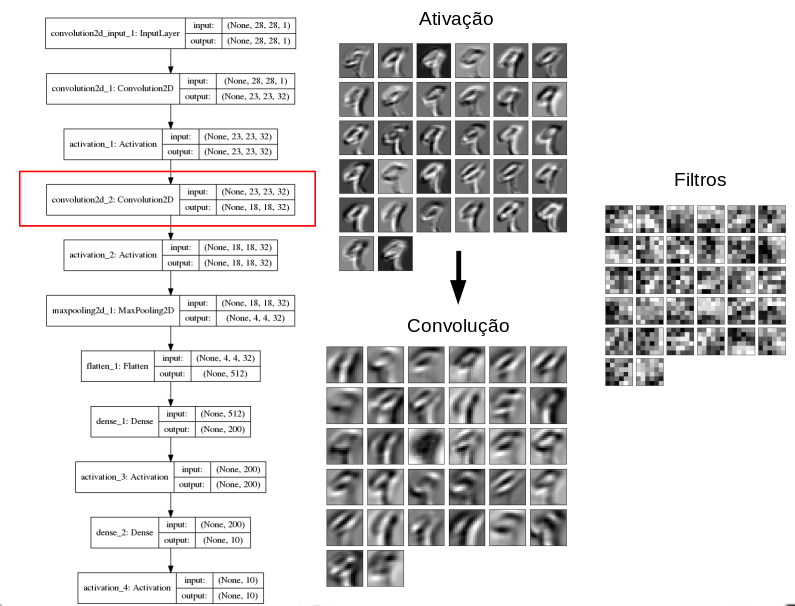
\includegraphics[width=.8\paperwidth]{images/fabio/conv_2}
\end{frame}

\begin{frame}
	\frametitle{Ativação - 2}
	\centering
	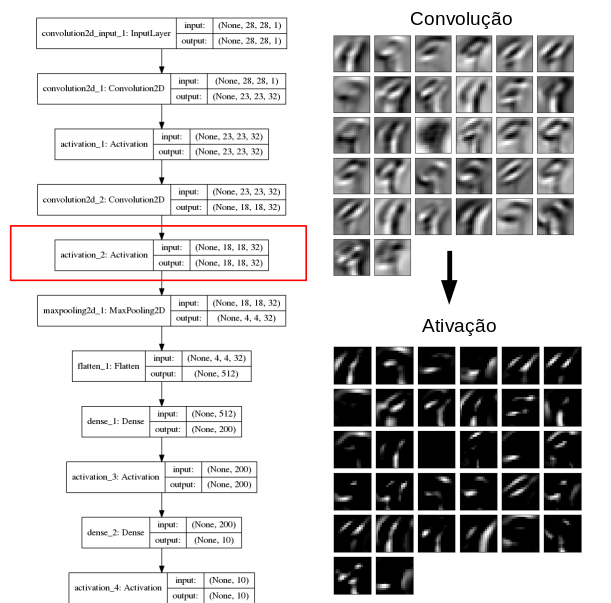
\includegraphics[height=.8\paperheight]{images/fabio/ativ_2}
\end{frame}

\begin{frame}
	\frametitle{Pooling}
	\centering
	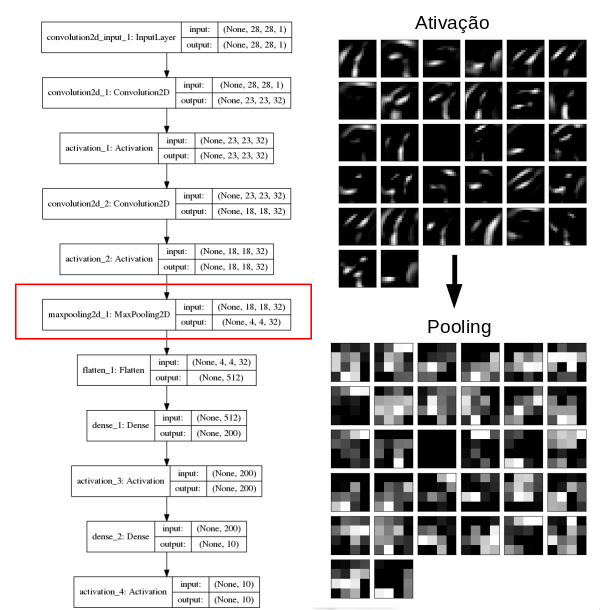
\includegraphics[height=.8\paperheight]{images/fabio/pooling_1}
\end{frame}

\begin{frame}
	\frametitle{Flatten ( N * 2D -> 1D)}
	\centering
	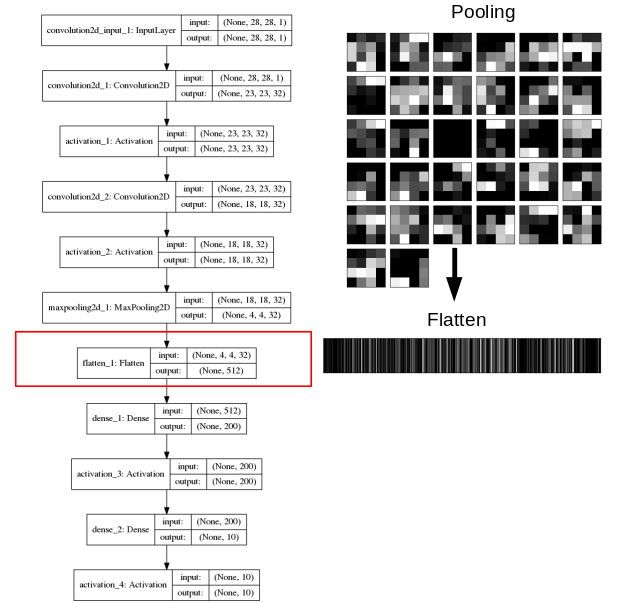
\includegraphics[height=.8\paperheight]{images/fabio/flatten_1}
\end{frame}


\begin{frame}
	\frametitle{Dense - 1}
	\centering
	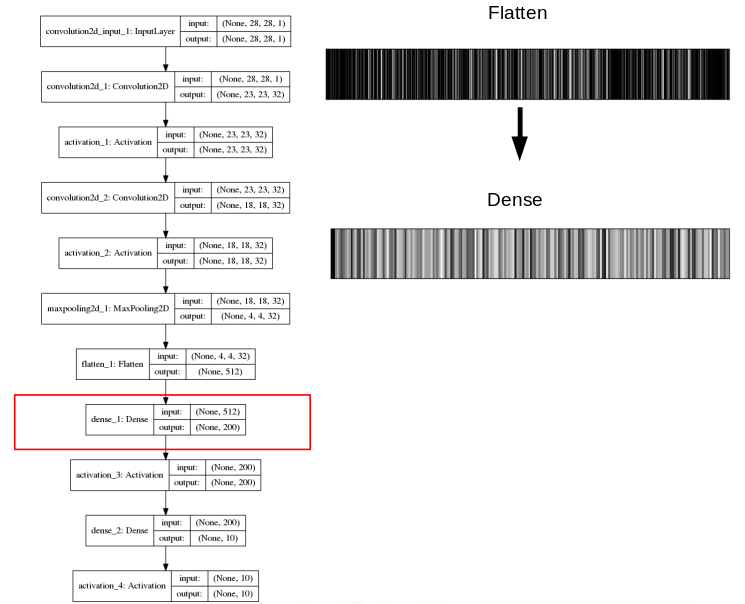
\includegraphics[height=.8\paperheight]{images/fabio/dense1}
\end{frame}

\begin{frame}
	\frametitle{Ativação - 3}
	\centering
	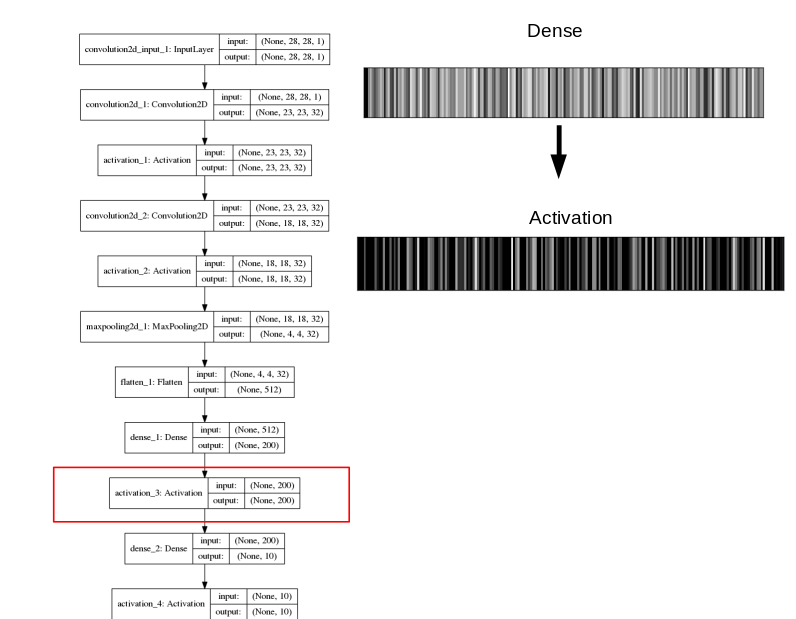
\includegraphics[height=.8\paperheight]{images/fabio/ativ_3}
\end{frame}

\begin{frame}
	\frametitle{Dense - 2}
	\centering
	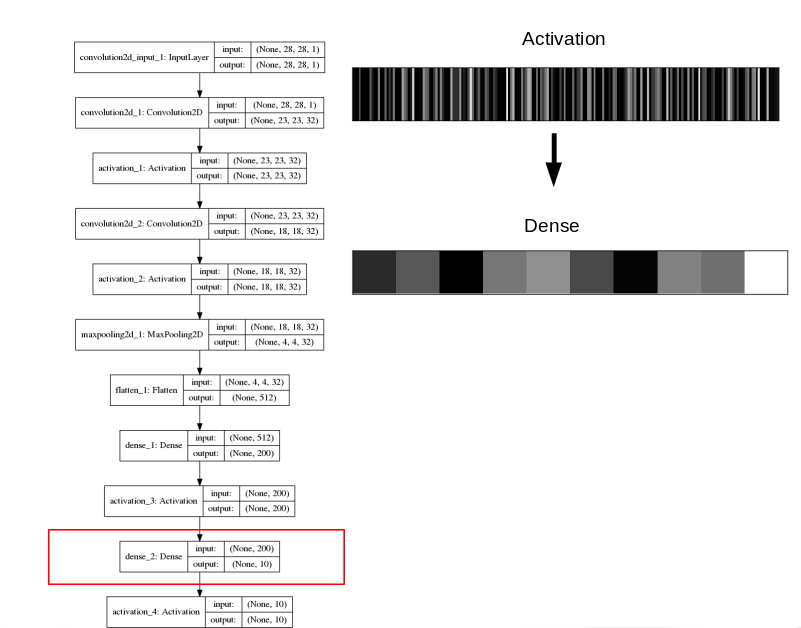
\includegraphics[height=.8\paperheight]{images/fabio/dense2}
\end{frame}

\begin{frame}
	\frametitle{Ativação - 4}
	\centering
	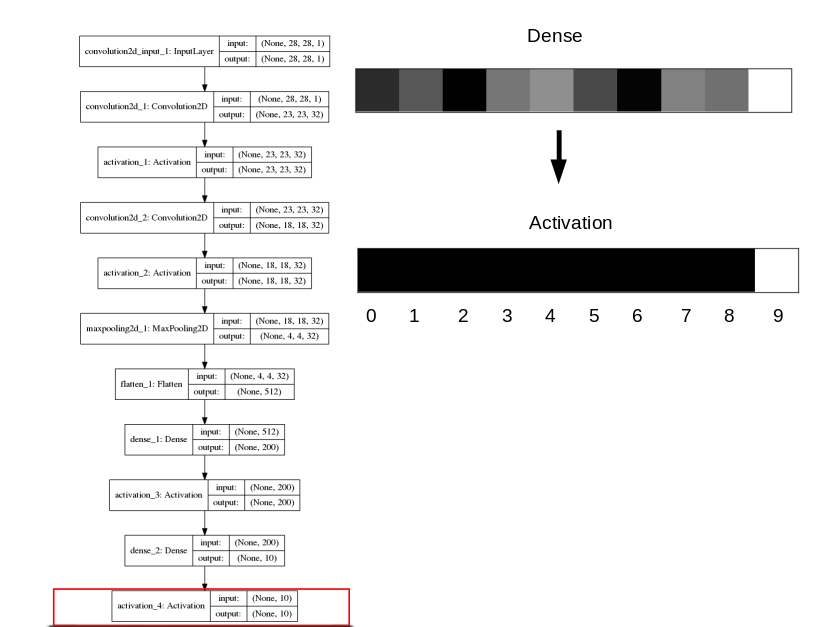
\includegraphics[height=.8\paperheight]{images/fabio/ativ_4}
\end{frame}


\begin{frame}
	\frametitle{Resultados das demais redes testadas - 1 }
	\centering
	\par Precisão na base de treino: 98.94\%
	\par Precisão na base de teste: 98.89\%
	\par 3 conv + 1 pooling + 3 conv + 1 pooling + 2 FC 
	\\
	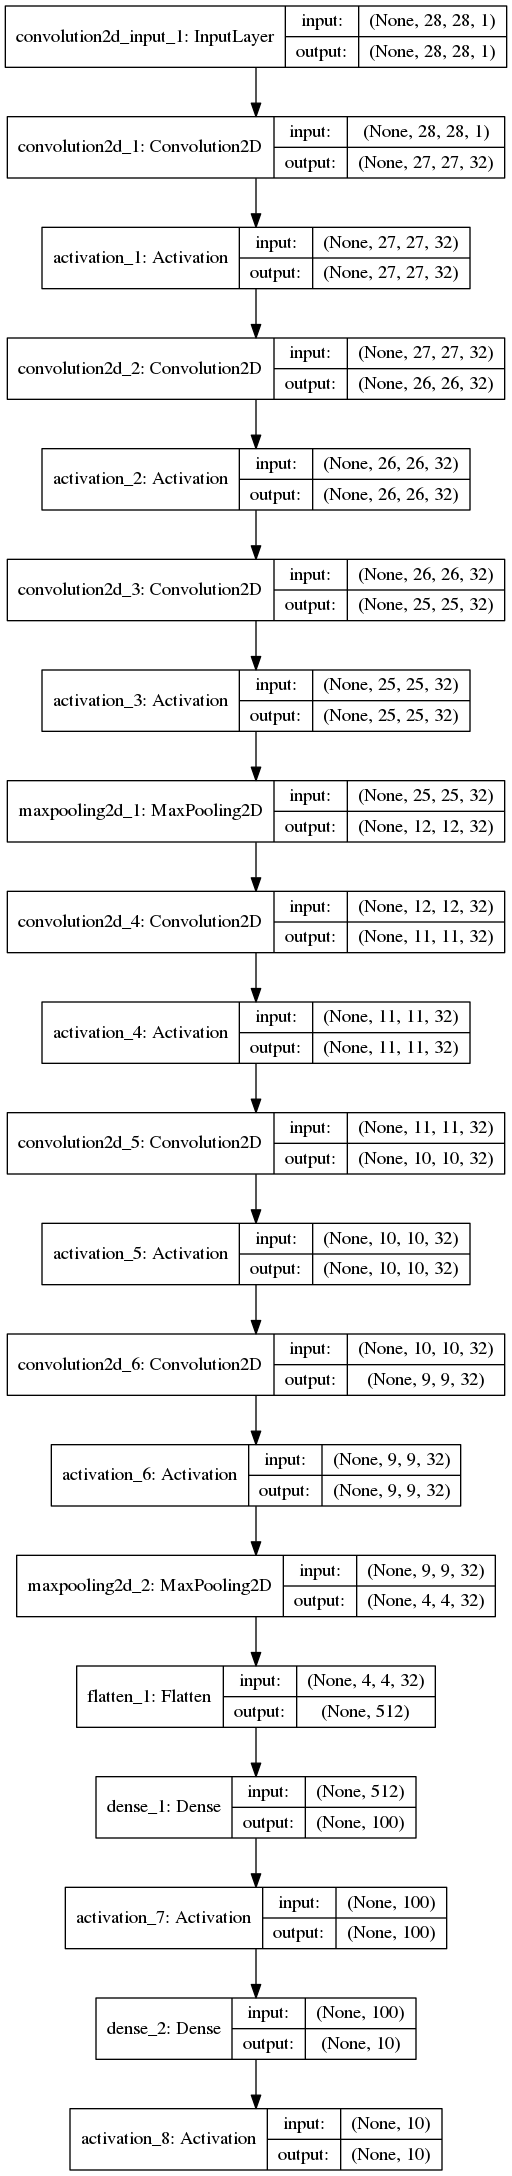
\includegraphics[height=.7\paperheight]{images/resultados/network_1/model}
\end{frame}

\begin{frame}
	\frametitle{Resultados das demais redes testadas - 2 }
	\centering
	\par Precisão na base de treino: 98.94\%
	\par Precisão na base de teste: 99.06\%
	\par 3 conv + 1 pooling + 3 conv + 1 pooling + 2 FC \(com dropout\)
	\\
	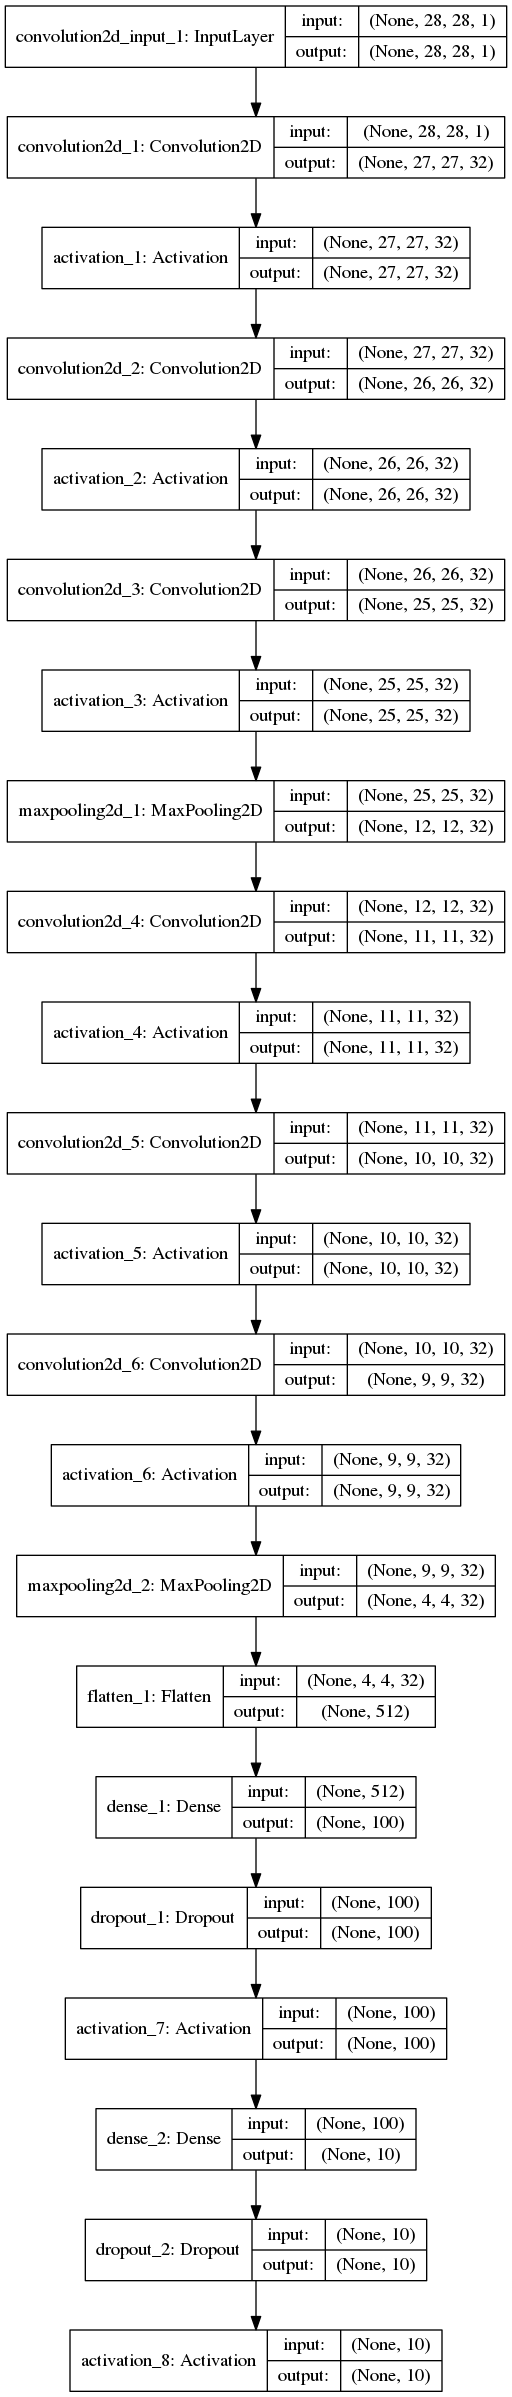
\includegraphics[height=.7\paperheight]{images/resultados/network_2/model}
\end{frame}

\begin{frame}
	\frametitle{MLP \& CNN}
	\centering
	\begin{itemize}
		\item CNN é uma extensão do conceito da MLP
		\item Convoluções e Pooling ajudam a diminuir rapidamente o número de variáveis do sistema
		\item Próprio para o processamento de imagens e vídeos		
	\end{itemize}
\end{frame}

% -------------------------------------------------
% end{fabio}
% -------------------------------------------------
\end{document}